\documentclass[paper=A4,pagesize=auto,11pt,headinclude=true,footinclude=true,BCOR=0mm,DIV=calc]{scrartcl}
\usepackage[english]{babel}
\usepackage[utf8]{inputenc}
\usepackage{graphicx}
\usepackage{geometry}
\usepackage[T1]{fontenc}
\usepackage{lmodern}
\usepackage{amsmath}
\usepackage[scaled]{uarial}
\usepackage{blindtext}
\usepackage{hyperref}
\usepackage{eurosym}
\usepackage{color}
\usepackage{subfigure}
\usepackage{listings}
\usepackage{float}
\usepackage{amsfonts}
\usepackage{amssymb}
\usepackage{graphics}
\usepackage{wrapfig}
\usepackage{setspace}
\usepackage[font=footnotesize]{caption}
\usepackage[format=plain,
justification=RaggedRight,
singlelinecheck=false]
{caption}
\usepackage{textcomp}
\geometry{
	left=2.5cm,
	right=2.5cm,
	top=2.5cm,
	bottom=2cm,
}
\makeatletter
\newcommand{\MSonehalfspacing}{%
	\setstretch{1.44}%  default
	\ifcase \@ptsize \relax % 10pt
	\setstretch {1.44}%
	\or % 11pt
	\setstretch {1.44}%
	\or % 12pt
	\setstretch {1.44}%
	\fi
}
\MSonehalfspacing
\setlength{\parindent}{0pt}

\begin{document}
	
	\title{Github Repository Classifier}
	\author{\textbf{Rami Aly$^{1}$, Andre Schurat}$^{2}$\\
		$^{1}$ University of Hamburg\\
		$^{2}$ Technical University of Dortmund}
	\maketitle
	
	\newpage
	
	\section{Abstract}
	
	
	\newpage
	
	\tableofcontents 
	
	\newpage
	\section{Selecting features} 
	\subsection{General thoughts}
	In the early beginning of our process we discussed about our selection of Features. We analyzed many repositories and  we realized that it is not possible for us to manually enclose the available data sets in a way where we woul not miss important features. For example if we choose Web sites produced by Jekyell as the indicator for the class WEB we will probably miss other Web applications as the software and the use-case market is to wide to manually find all necessary features. So we decided to not cut down the data sets, instead we condoned gathering statistically irrelevant informations so far. In the further context we will call this phenomena “information noise”.
	\subsection{Selected features}
	For a better visualization of  created a graphic:
	\\
	INSERTPICTURE
	\\
	The entries with a double circle represent our features. In the further process we explain our decision to choose this ones and why we didn’t choose other.
	Why we choose these features and didn’t choose other ones will be explained in detail in the further process.
	
	The next section is used to explain our decision behind our feature selection, and why we didn’t use other ones, although we considered them. 
	
	\subsubsection{Word Count}
	The word count represents our most important feature. It is defined as the occurrence of each word contained in any text across the whole repository. This includes all readable text files, and text contained in PDF, Word and Powerpoint files. The contents of the readme file count 10 times as much since it contains the most important information the most cases. 
	We choose this feature because the Word Count represents the repository’s content in really wide way. At this point we keep in mind that at the backside the information noise especially for the word count is immense. 
	An example of a Word Count Table can be found inside the attachments. TODO
	
	\subsubsection{File Ending Count}
	
	The File Ending Count is defined as the occurrence of different file endings in the whole repository. We choose this feature because file endings reflect the use of different programming languages and other file formats in the best possible way.
	
	\subsubsection{Filename Count}
	
	Just like the File Ending Count the Filename Count is defined as the occurrence of different file and folder names in the whole repository.
	We choose this feature because there are several key files and folders which militate in favor of a specific category.        
	
	\subsubsection{Media Density}
	
	The Media Density describes ratio from the total count of media files to the total word count contained inside the Word Count. Media files contained inside PDF, Word. Zip and Powerpoint files are counted as well. We choose this feature because there are specific repository categories that tend to use more or less media files.
	
	\subsubsection{Average File Size}
	This feature is mostly used to detect the ratio between file number and its size. This feature correlates with the Media Density but it is mainly used to detect big crowed files. This would rather indicate a DOC or EDU class than the OTHER or DEV class.
	
	\subsubsection{Number Density}
	Firstly we did not thought about this feature. But as we build our \hyperref[sec: dictionary]{dictionaries} we noticed that occurrences of numbers varies greatly between the classes. Thus we decided to use a feature to merge every number: the Number Density.
	
	\subsubsection{Commit messages}
	The use of commit messages and commits in general was a bit problematic. While we seriously thought about using this as a feature but commit messages are too variable to it. It would be like trying to interpret the interpretation of information so the possiblity to classify repository wrongly based on the messages is not as small as we wish it too be.
	
	
	Furthermore available data by a simple web browser is huge but since not of all it may accessible via code we took a look into the Github API instead. This offered a major problem: The Github API only allows 60 unauthenticated requests per hour and 5000 for authenticated ones(1). Even if we take into count that only authenticated requests are used, which would require each user to own a github account, 5000 requests per hour are not enough to analyze hundreds of Repositories per hour. There are  Repositories with over 500.000 commits and a single github request returns only the first 500. So we would need 1000 request for a single repository just to get all of the commits.
	
	\subsubsection{E-Mail of repository owner}
	This feature is problematic. We thought about searching for an edu substring in the email but we could not find a correlation with the EDU class. Apart from this we could not think of any part in an e-mail which could be relevant.
	
	
	
	
	
	\section{Gathering selected features from Github}
	
	\subsection{Gathering the Repository’s content from Github}
	
	\subsubsection{Choosing the content acquiring method}
	
	To gather the Repository’s contents you would normally request the File Tree which represents a lists off all available files including their size, their name and their download link. If a file should be further analyzed in detail, you can get it’s content via File Tree’s download link.\footnote{\url{	https://developer.github.com/v3/git/trees/get-a-tree-recursively}}
	
	The main issue using this method is the previously mentioned Rate Limit of Github’s API. Requesting each file that should be analyzed individually results in a hundreds of request per repository.
	So instead of requesting each file on it’s own, there is the option to grab whole content as “zipball”. On the one hand this results in only one request per repository and the content is already compressed, on the other hand we may grab a files that we are not going to analyze at all. 
	But we could  additionally observe that the zipball requests aren’t limited 60 unauthenticated ones per hour. Which makes grabbing the “zipball” superior to requesting the file tree. This way our classifier does not need any form of authentication and our classification performance if only limited to our network bandwidth and the hardware of the operating system.
	
	\subsubsection{ Grabbing the “zipball”}
	
	
	The resulting downstream of the grabbed "zipball"\footnote{Request: \url{https://api.github.com/repos/username/repositoryname/zipball}} is inflated on the fly into multiple virtual files. A virtual file describes a file that is not written onto hard disk, instead is it kept inside the classifier’s heap. This results in a huge RAM usage but allows much faster processing of the gathered files.
	
	\subsection{Categorizing Files}
	
	In the next step all virtual files are categorized into the following eight different categories: Zip, PDF, Word, PowerPoint, Text, Binary, Image and Folder. The category where a file belongs is determined by a fixed procedure. 
	At the beginning it is checked if the is a folder. If it is not we use arimus’s jmimemagic libary https://github.com/arimus/jmimemagic to get the file’s Internet Media Type (MIME-Type). If a the MIME-Type can’t be parsed from the file, there is still a chance that the investigated file could be a readable text file. To avoid missing such files we use an additional method to guess whether or not the file is a readable text file. The method basically calculates ratio between the amount of ascii bytes and other ones. If the ratio of non ascii bytes is greater than 5% we assume the file is not a readable text file. Nevertheless we don’t rely on this method neither on the MIME-Type. Instead we use both in combination with the file’s extension, to make the final decision in which category a file belongs. If a file falls into either the Binary or the Image category its content stored inside the heap gets released, since we can’t analyze these files further.
	
	\subsection{Inflating the Filelist}
	
	The Zip Category contains all type archives that are Inflatable. We think a lot of information can be hided inside those, we inflate them, and they undergo the same procedure like the “zipball”. The recursive depth of this method is one so archives inside archives files inside zip files are not analyzed. The reason behind this decision is on the one hand the performance impact and on the other hand we don’t think that files gathered by a deeper recursion would be relevant for the repository’s type.
	
	\subsection{Getting Word Count}
	
	\subsubsection{ Access non readable files that contain text}
	To extract the Word Count out of the Inflated filelist, we need to access to the text contained in the non readable text files. To extract it out of PDF files we use Apache’s PDFBox library inside a simple wrapper class, which allows us to extract the raw unformatted text out of pdf files. For the Microsoft’s PowerPoint and Word files, we use Apache’s POI library, in a similar way.
	To avoid opening any file twice we also extract the amount of Media Files inside the analyzed files. 
	
	
	
	\subsubsection{Formatting the raw text}
	To get as many matches as possible, we  normalize the the raw text. To    accomplish this we remove first of all, all hyphens followed by a line break. This way we can restore any word that was splitted due to a line break. Afterwards all line breaks are replaced with a whitespace. This is needed because the Scanner we use to parse single words form the normalized text uses a whitespace as delimiter. In the next step we replace all non ascii letters with ascii ones. This would convert the following String “äèôãç” to “aeoac”. This step is needed because in the next step, all non ascii and other special characters are being removed.
	
	
	\section{Removing irrelevant information from selected features}
	\label{sec: dictionary}
	\subsection{Algorithm to create Dictionaries}
	Especially the features \textit{File Ending Count}, \textit{Word Count} and\textit{ Filename Count} still consists of information noise as every repository could contain words that are unique to every other repository and are as such not relevant for the classification. Then again some words could be in almost every repository but their occurrence does not differentiate between the classes in a considerable margin. Due to the rising complexity of a neural network for every input added to it one should desire to find a balance between the number of words and the relevance of a word for classification. We decided to create a dictionary for each of the mentioned three features that contains every relevant word for classification.
	Of course the question arises on how to chose the words for the dictionaries. For this we created an algorithm.
	
	The algorithm takes classified repositories, we choose to use our \hyperref[src:Repositories]{Training Datasets}.
	In the first step the intersection with a threshold $p$ of words between repositories of the same class is calculated for each repository class. The threshhold $p$ is used to define the minimum ratio between repositories that contain the word and the total number of repositories in the class. 
	This step is used to filter words that are too unique.
	
	In the next step the ratio between the occurence probability of a remaining word in a class and the average occurence of a word over \textit{all} repositories is calculated for every word and class. We will thus sort the seven (in case we have seven classes) Lists from large to small  This step is used to find the words with the highest deviation from the average occurrence and therefore helps to classify a repository. Combined with the first step we thus selected words that exist in many repositories and their occurrence probability is highly dependent on the class of the repository.
	Our dictionary is than created by adding he first $q$ words of a list of each class to a set (because words can exists in multiple lists).
	\begin{figure}[H]
		\subfigure{\label{konfiguration}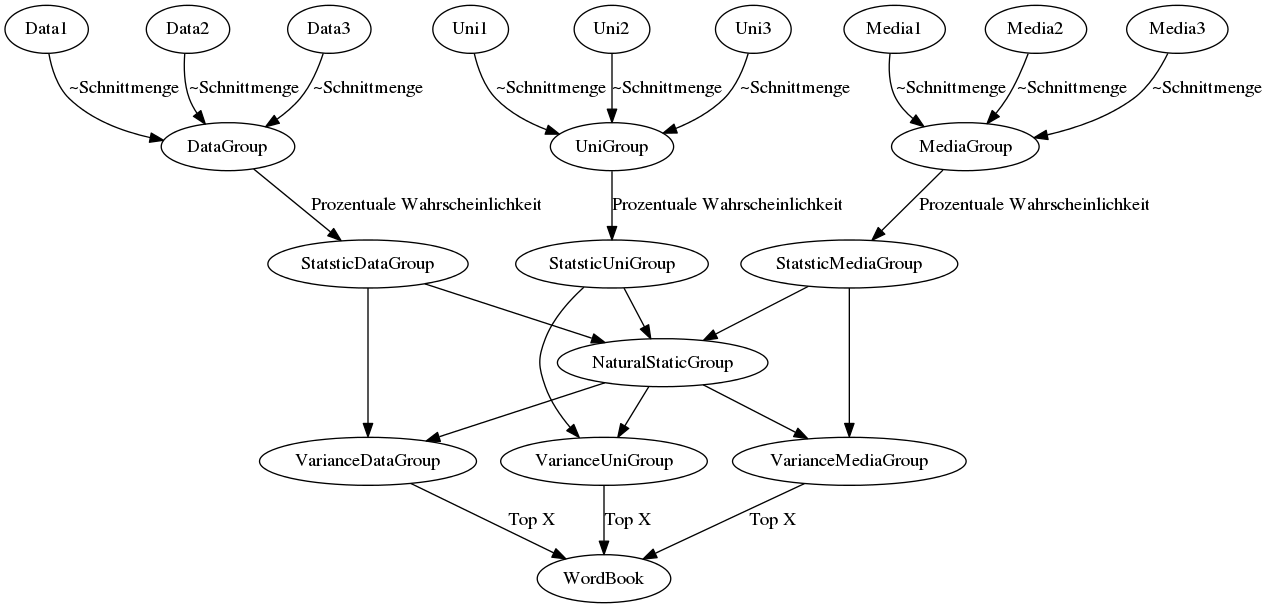
\includegraphics[scale = 0.35]{images/Woerterbuchbildung.png}}
		\caption{Dictionary calculation visualized}
	\end{figure}
	
	\subsection{Created Dictionaries} 
	So the next important step is to chose $p$ and $q$. At this point we have to note that we did not try to chose the dicitonaries as we \textit{think} they are good by just watching over the selected words.
	But rather tried to use the information we know about the words and their deviation to generate it. We tried to calculate the optimum between number of words and deviation as well as occurrence probability.
	These are the resulting three dicitonaries and as such the dicitonaries with less information noise:
	\\
	INSERT DICTIONARY
	\\
	
	\section{Building the Prediction Model}
	
	\subsection{Choosing a prediction Model}
	Of course there are many different approaches to the problem. A static algorithm to classify repositories is rather impractical because the parameters of our classify function would be strongly influenced by our interpretation of weights of the features for each class. However we quickly noticed that the complexity is very high, so that a normal algorithm would limit the aspects which possibly needed be considered. The problem is non-linear and through the static analysis we would loose the possibility to freely improve or change the classifier. As the software and use-case market of Github rises the possible need of further classes could arise.
	
	Hence to ensure a classifier who is as dynamic and as extensible as possible we choose to use some form of machine learning.
	The problem which needs to be solved by the Prediction Model is a classification problem: We have a fixed number of values for selected features as input and as an output the class to which the values fit the most. As a result of this fact it was pretty clear to us that a supervised learning method would be optimal.
	
	In the next step we thought about the pro- and contra arguments of non-parametic and parametic learning.
	For example Gaussian-Process-Models could be used in principle, as one does not need to specify a fixed number of parameters and therefore be non-parametic. 
	The main problem with Gaussian-Process-Models is that they scale rather poorly with a complexity of $O(n^{3})$ \cite{DukeUniversity}. Moreover if we keep the huge dimension of repository datasets in mind and as such the possible complexity of the classifier function, our choice will lead us to a parametric neural Network. A neural network combines every important aspect from above and is furthermore capable of performing good in presence of imprecise and especially of noisy data.
	
	\subsection{Our Neural Network Model}
	First of all for our selected features it is not needed to consider temporal behavior. We do need need to save an internal state (If we had used a sequence of commits this could have been otherwise). It should be fully sufficient to use a Feed-forward neural network.
	
	As for a Neural Network with supervised learning we choose that a Multilayer perceptron(MLP) with one hidden Layer would be sufficient for our classification problem. We already mentioned that our classification problem is not linear. Hence at least one hidden Layer is required to solve the problem. Furthermore we know that this MLP can approximate any bounded continuous function with arbitrary precision \cite{ApproximateAnyFunction}, particularly our classification problem.
	The usage of a linear activation function would result in a MLP with a set of possible functions to be equivalent those of a normal input-output perceptron. Therefore we needed to use a nonlinear activation function. We thus decided to use a Sigmoid function. 
	
	For the training we used Backpropagation as expected for a MLP. To reduce the chance to be stuck in a local minimum we used inertia so that the previous change will influence the weight adjustment in the current round.
	
	The neuron count for the output-layer is set to the number of different classes into which we want to classify the input. So for our Neural Network we used seven output neurons.
	
	Our input neurons count equals to sum of the length of every dictionary plus all relevant ratios of our selected features.
	
	\subsection{Formating and further preprocessing of Features to fit into the Neural Network}
	We tried to find the perfect balance in preprocessing so that on the one hand the network does not need to learn obvious relations between features and on the other hand does not to loose possible relations by too much preprocessing.
	
	To format the input for the neuron we will iterate through every word in a dictionary of a type. The ratio between the relative occurence of the word for this type and the occurence value stored in the dictionary is calculated. Effectively this ratio is equal to the deviation of the relative word occurrence for the considered type. In case the relative occurrence of a word ending is higher then the occurrence in the dictionary it will result into a value $> 1$. So there is still the necessity of a normalization process - for the dictionary deviation as well as for the ratios.
	
	There are several possibilities to normalize the input. In our case it is important that the input is distinct. Furthermore standard normalize procedures are using a maximum and minimum value. The problem is that it is not possible to define an upper bound for the inputs because a testinput could always exceed the previous bound and therefore the attribute of distinction is contradicted in case the input should still be normalized (New Max value could lead to values to have the exact same value as a value with an old bound). Nonetheless we tried the different normalization procedures of min-max normalization and standardisation but the \hyperref[src:optimizing]{results} results (\hyperref[src:optimizing]{Chapter 5.4}) were rather disappointing.
	
	
	Therefore we decided to use a logistic function to normalize our data. A logistic function is monotonically increasing and thus is every value distinct. Depending wether we use a Sigmoid or tanh function we will construct the logistic function in a way that the upper bound is 1 and the lower bound respectively 0 or -1 in case of the tanh. 
	We can then use a constant of proportionality to optimize the distribution of the values:
	
	$f(x) = 2 * \frac{1}{1 + e^{-k(x-k)}} -1$
	
	To support the understanding of our normalization technique we will plot our function for $k \in \{0.03, 1, 5\}$.\\
	\begin{figure}[H]
		\subfigure{\label{konfiguration}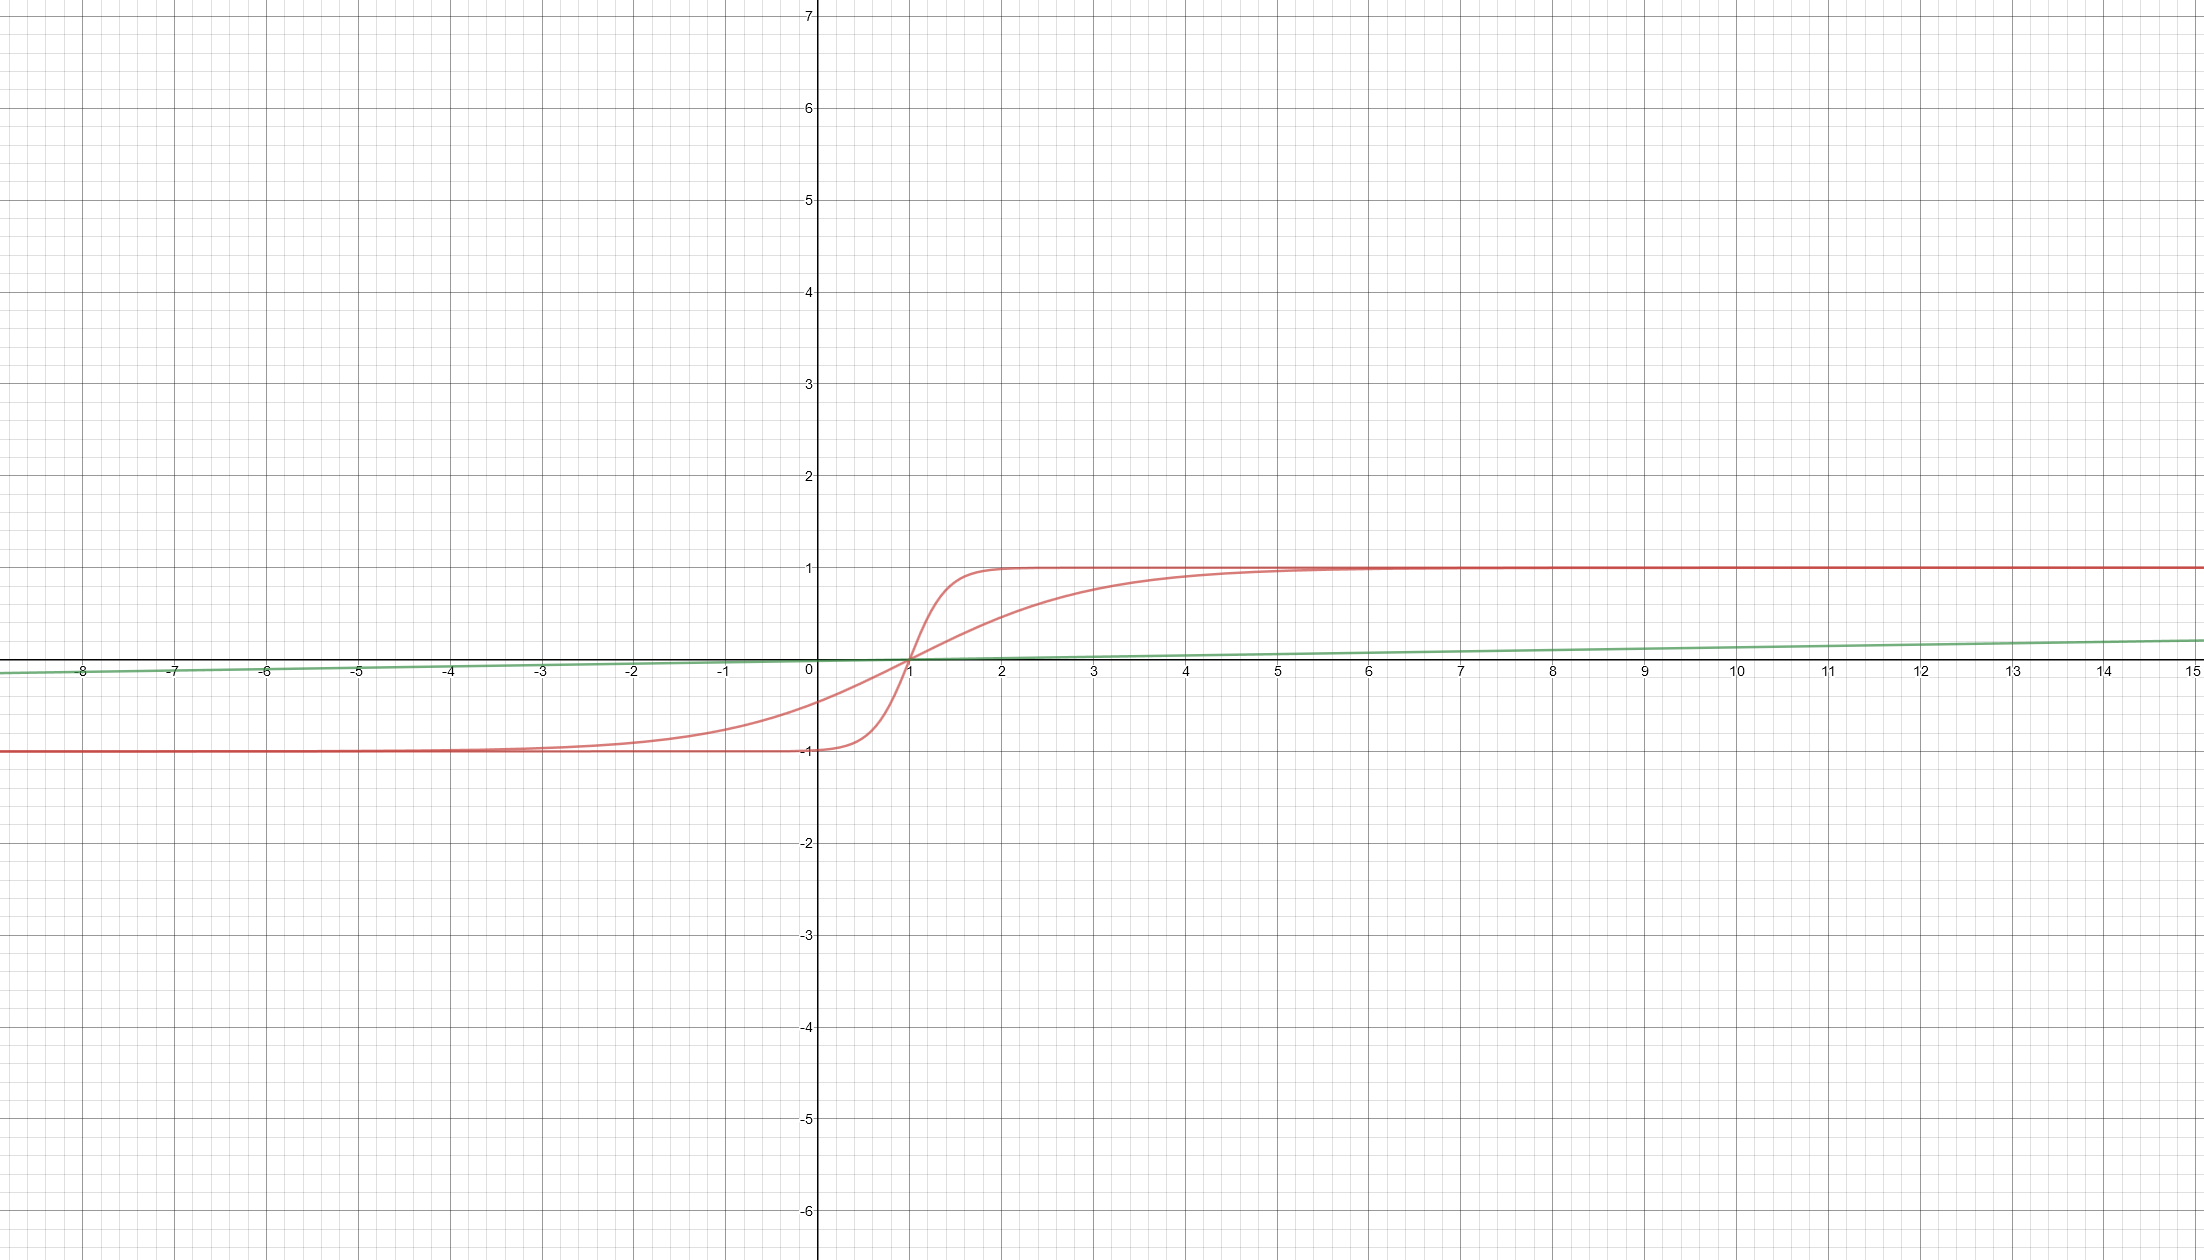
\includegraphics[scale = 0.2]{images/logistic.png}}
		\caption{k = 0.03 in green, k = 1 in bright red, k = 5 in red}
	\end{figure}
	
	The normalization process will take place for every dictionary and ratio but they all have to define their own proportional constant.
	Every value is stored as a double and the index position of the features a static.
	
	
	
	
	
	\subsection{Data Sets and Training}
	Beside the labeled repositories in the challenge description we used \hyperref[src:TrainingRepositories]{most} of the the additional \hyperref[src:Repositories]{Repositories} provided by a participating team in the official github repository of the InformaticCup 2017 as training repositories (although you cannot read it: a big thank you at this point!). We have to admit that even as a human being the classification is not as clear as we thought it would be. Sometime we were not sure if the labeling of the data Sets we used were correct and we realized that many repositories overlap with different categories and it is not always objectively clear to which repository it fits more. In this case the repositories were labeled by personal preference and estimation. Therefore the learning of our network is influenced by personal decisions as it uses the labels.
	
	Since we are using backpropagation after each iteration the actual output of the network is compared to the desired output and using the euclidean distance leads us to an error value. Update the parameters of the classification function(in this case the weights of the neural network). The Training continues until this error value is below a manual set value.
	
	
	
	\section{Optimizing our Neural Network }
	\label{src:optimizing}
	A potentially very time consuming task is to optimize the network. We divided the possible optimizing parameters into three categories. Firstly we need to optimize the training. Besides changing the inertia and learn rate it is far more important to take care of the error value of the neural network. A min error value far to low could result into over fitting the neural network to the repositories of the training phase. Then again a min error value too high would result into a very unstable Network and an under fit network. 
	The second category would be optimizing the features selected in the beginning. We have to consider that our selected features are not as optimal as expected.
	Lastly we need to optimize the neural network itself. This counts in the hidden Layer as well as the preprocessing step of normalizing the values.\\
	For Testing we used the Test Repositories given by the Challenge Description. To prevent an over fitting on the Test repositories we decided to use further ones provided by the additional Dataset for testing. We used further 36 Repositories (6 per class) so all in all we tested our neural network on 67 \hyperref[src:TestRepositories]{Repositories}.  We thought about different testing methods for testing. Known procedures like k-fold cross validation do not have benefints in our case because in our opinion the dataset is not big enough for this. There is a natural deviation in results in each change of a parameter and it is not easy to tell wether this change has been random or has really improved the network. The rather small datasets we would obtain for k-fold cross validation would increase this problem while reducing the possible over fitting. Nontheless we decided to stay with our fixed 67 repositories.
	The base values resulted to following results
	GANZ VIELE MESSDATEN(VERTEILUNG DER OUTPUTS, ABSOLUTE TREFFER ETC......)
	The parameters we changed too modify are the number of hidden Layer, the neurons in each hidden Layer, the Values $p$ and $q$ for the dictionary, the weight of the Readme words and the proportional constant $k$ for our defined logistic function.
	We firstly changed the $k$ values as they are not as variable as the other values. We just need to find a value so that the function distributes the input values even. This could be done by calculating the average distance between the values.
	Based on the first results of our network we decided to vary the count of Neurons in the hidden Layer.
	
	\section{Validation of created Classifier}
	-> Hängt vom Usecase ab
	<gleiche anzahl an repo für jeden typ
	-> Suchfunktion mit Eingerzung und Filter Lieber hohe Ausbeute(nichts verpassen was wichtig ist)
	-> Umso höher die Anzahl der betrachteten Repositories ist, umso wichtiger präzision(also richtige einordnung wichtiger wenn man generell viele repoos betrachten möchte)
	->geringer, dann Ausbeute(siehe punkt 1)
	
	
	->Vorgehen
	
	->Präz und ausbeute berechnen
	->Indizien für schwach oder stärken unseres Netzes
	->Sagen was wichtiger ist
	-> Verbesserungen
	
	\section{Possible improvement approaches}
	
	\section{Extensions}
	
	
	\newpage
	
	\begin{thebibliography}{xxxxxx}
		\bibitem [1] {DukeUniversity} David P. Williams Gaussian Processes (2006) \url{http://people.ee.duke.edu/~lcarin/David1.27.06.pdf}
		\bibitem [2] {ApproximateAnyFunction}  Cybenko., G. (1989) "Approximations by superpositions of sigmoidal functions", Mathematics of Control, Signals, and Systems \url{http://deeplearning.cs.cmu.edu/pdfs/Cybenko.pdf}
	\end{thebibliography}
	
	
	\section{Source Code, used external Libraries and Repositories}
	\paragraph{Source Code}
	Github: \url{https://github.com/Crigges/InformatiCup2017}\\
	\paragraph{Repository Dataset}
	\label{src:Repositories}
	\url{https://github.com/InformatiCup/InformatiCup2017/tree/master/additional_data_sets}	\\
	
	\label{src:TrainingRepositories}
	\paragraph{Training Repositories}
	Exact repositories used fo training can be found in the document TrainingRepositories.
	
	
	
\end{document}



